\documentclass[]{scrartcl}
\title{Vorlesung Analysis II}
\usepackage{amsmath,amssymb,amsfonts}
\usepackage{stmaryrd}
\usepackage{mathtools}
\usepackage{latexsym}
\usepackage{graphicx}
\usepackage{tikz}
\usepackage{xcolor}
\usepackage[most]{tcolorbox}
\usepackage{soul}
\usepackage{ upgreek }
\usepackage{hyperref}
\usepackage{tipa}
\usepackage[dvipsnames]{xcolor}
\hypersetup{
	colorlinks=true,
	linkcolor=blue,
	filecolor=magenta,      
	urlcolor=cyan,
	pdftitle={Overleaf Example},
	pdfpagemode=FullScreen,
}
\newcommand{\redcircle}[1]{%
	\tikz[baseline=(char.base)]{
		\node[shape=circle, draw=red, text=red, thick, inner sep=1pt] (char) 
		{\textbf{#1}};
	}%
}
\newcommand{\bluecircle}[1]{%
	\tikz[baseline=(char.base)]{
		\node[shape=circle, draw=blue, text=blue, thick, inner sep=1pt] (char) 
		{\textbf{#1}};
	}%
}
\newcommand{\blackcircle}[1]{%
	\tikz[baseline=(char.base)]{
		\node[shape=circle, draw=black, text=black, thick, inner sep=1pt] 
		(char) 
		{\textbf{#1}};
	}%
}
\newcommand{\orangecircle}[1]{%
	\tikz[baseline=(char.base)]{
		\node[shape=circle, draw=orange, text=orange, thick, inner sep=1pt] 
		(char) 
		{\textbf{#1}};
	}%
}
\newcommand{\redul}[1]{\setulcolor{red}{\ul{#1}}}
\newcommand{\blueul}[1]{\setulcolor{blue}{\ul{#1}}}
\newcommand{\yelul}[1]{\setulcolor{yellow}{\ul{#1}}}
\newcommand{\greenul}[1]{\setulcolor{green}{\ul{#1}}}
\newcommand{\oraul}[1]{\setulcolor{orange}{\ul{#1}}}
\setul{1pt}{3pt} % Linienhöhe und Abstand zum Text (optional anpassbar)

\setlength{\topmargin}{-.5in} \setlength{\textheight}{9.25in}
\setlength{\oddsidemargin}{0in} \setlength{\textwidth}{6.8in}
\setlength{\parindent}{0pt}

\begin{document}
	\maketitle
	\textbf{\underline{Teil 1: Differentialrechnung im $\mathbb{R}^n$}}\\
	\\
	\textbf{\underline{an9: Extrema mit Nebenbedingungen, implizierte 
	Funktionen}}\\
	\\
	\textbf{\underline{\underline{Stichworte:}Extrma mit NBen, 
	Lagrange-Multiplikationen, implizierter Funktionensatz}}\\
	\\
	\textbf{\underline{Literatur}} \blueul{[Hoff], Kapitel 9.8, [Forster], 
	Kapitel 8,9}\\
	\\
	\textbf{9.1. \underline{Einleitung:}} Sla Anwendung des Satzes von der 
	lokalen Umkehrbarkeit zeigen wir den impliziten Funktionensatz und 
	untersuchen Extrema mit Nebenbedingungen.\\
	\\
	\textbf{9.2 \underline{Motivation:}} Sei $a \in U\subset \mathbb{R}^n, 
	f:U\rightarrow \mathbb{R}$. Diskutieren im Fall \underline{n=2:}\\
	\underline{1. Ziel:} Wollen die Glg. f(x,y)=0 "nach y auflösen", also eine 
	Fkt. l finden mit \greenul{$f(x,y)=0\Leftrightarrow y=l(x)$}. Wir sagen 
	dann, die Glg. f(x,y)=0 definiert \underline{implizit} eine FUnktion l. Wie 
	und unter welcher Vor. das geht, beschreibt der Satz über implizite 
	Funktionen. Wir erwarten, das dies nur "lokal" geht, also auf Umgebungen 
	einer Stelle a und einem Wert b mit f(a,b)=0.
	\begin{figure}[h]
		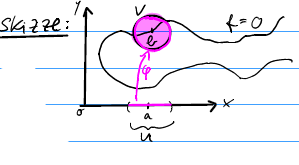
\includegraphics[width=5 cm,height=3cm]{bsp kap 9.2}
	\end{figure}\\
	\underline{Konkretes Bsp.:} Glg. $x^2+4y^2=1 \rightarrow 
	f(x,y)=x^2+4y^2-1$, und $y= \pm \frac{1}{2}\sqrt{1-x^2}.$\\
	\underline{2. Ziel:} Bsp. \underline{n=2}\\
	In Anwendungen er Extremwertbestimmung wird oft nach Extrema von Funktionen 
	g(x,y) auf einer \redul{Nullstellenmenge}\yelul{N}$:=\{(x,y)\in \mathbb{R}^2; 
	f(x,y)=0\}$ gefragt, d.h. \greenul{unter der Bedingung f(x,y)=0}. Gegeben 
	ist dann eine \redul{"Nebenbedingung"}.\\
	\underline{Konkretes Bsp.:} $\overline{f}(x,y)=\frac{xy}{1+x^4+y^4}$, ist 
	stetig, nimmt Extrema auf $N=\{(x,y);f(x,y)=0\}$ an. Ist $\begin{pmatrix}
		x_0\\y_0
	\end{pmatrix}\in N$ so eine Stelle, und ist $\begin{pmatrix}
		-1\\0
	\end{pmatrix}\neq\begin{pmatrix}
		x_0\\y_0
\end{pmatrix}\neq\begin{pmatrix}
		1\\0
\end{pmatrix}$, dann gilt nahe $\begin{pmatrix}
		x_0\\y_0
\end{pmatrix}: D_2f(x,y)\neq 0$.\\
	\begin{figure}[h]
		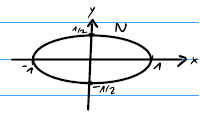
\includegraphics[width=5 cm,height=3cm]{bsp kap 9.2.2}
	\end{figure}\\
	\\
	\textbf{9.3. \underline{Allgemeine Situation:}} Sei $D\subset \mathbb{R}^n, 
	2\leq l \leq n, (f_1,...,f_l)=f\in l^1(D,\mathbb{R}^l)$.\\
	Setze \redul{$N:=\bigcap_{1=2}^l f^{-1}_i(0)$}, ist offen in 
	$\mathbb{R}^n$,\\
	Sprechweise: $f_1$ hat ein \redul{lokales Etremum in $a\in N$} mit 
	\redul{Nebenbedingung N}, falls $f_{1/N}$ in a ein lokales Extremum hat.\\
	\\
	\textbf{9.4. \underline{Satz:}} Geg. die \blueul{Situation 9.3}, 
	\underline{Vor.:} $f_{1/N}$ hat \greenul{in $a\in N$ ein lokales 
	Extremum}.\\
	\underline{Beh.:} rg $\begin{pmatrix}
		D_1f_1&\cdots&D_nf_1\\
		\vdots&&\vdots\\
		D_1f_l&\cdots&D_nf_l
	\end{pmatrix}(a) \textless l.$ \redul{"Lagrangesche Multiplikatorenregel"}\\
	\\
	\textbf{9.5. \underline{Bem.:}} $\bullet$ Im Fall l=n ist die Beh. 
	äquivalent zu $\begin{pmatrix}
		D_1f_1&\cdots&D_nf_1\\
		\vdots&&\vdots\\
		D_1f_n&\cdots&D_nf_n
	\end{pmatrix}(a)=0.$\\
	$\bullet$ Es gilt: Beh. $rg(...)\textless l$\\
	$\Leftrightarrow f_1'(a),...,f_l'(a)$ sind Lin. abh.\\
	$\Leftrightarrow \in (\overline{\lambda_1},...,\lambda_l)^T 
	\in\mathbb{R}^l\backslash\{0\}. 
	D_j(\sum_{i=1}^{l}\overline{\lambda_i}f_i)(a)=0$ für alle 
	$j\in\{1,...,n\}$.\\
	\OE sei $\lambda_1=1$(sonst unnumerieren und normieren).\\
	Also $\exists(\lambda_2,...,\lambda_l)^T\in\mathbb{R}^{l-1}$ mit 
	$D_jf_1(a)=\sum_{i=2}^{l}\lambda_iD_jf_i(a),$ alle $j\in\{1,...,n\}$.\\
	$\Rightarrow f_1(a)=\sum_{i=2}^{l}$\yelul{$\lambda_i grad 
	f_i(a)$}.\textopencorner \OE Ohne Minus vor den $\lambda_i$...\textcorner\\
	\textopencorner Bsp. für $l=2: \exists \lambda\in\mathbb{R}:grad 
	f_1(a)=\lambda grad f_2(a),$ für $f_2'(a)\neq 0$.\textcorner\\
	\\
	\textbf{9.6. \underline{Def.:}} Man nennt die $\lambda_2,...,\lambda_l$ 
	\redul{Lagrargemultiplikatoren}.\\
	\\
	\textbf{9.7. \underline{Bew.:}} Sei $\OE a = 0$. $\bullet$ Ferner betr. 
	zunächst den Fall \underline{l=n}.\\
	\underline{Angenommen}, es wäre sonst \oraul{rg A=n}, wo $\begin{pmatrix}
		D_1f_1&\cdots&D_nf_1\\
		\vdots&&\vdots\\
		D_1f_n&\cdots&D_nf_n
	\end{pmatrix}(0)\in\mathbb{R}^{nxm}.$\\
Dann ist \oraul{A eine invertierbare Matrix.}\\
	Der \blueul{Satz über lokale Umkehrbarkeit 8.8} liefert dann:\\
	$\exists U \subset \mathbb{R}^n \exists V \subset \mathbb{R}^n, o \in U, 
	f(o)\in V, U\xrightarrow{fru} V$ invertierbar und bijektiv.
	\begin{figure}[h]
		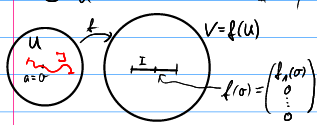
\includegraphics[width=5 cm,height=5cm]{bsp kap 9.7}
	\end{figure}\\
	Betr. \oraul{I:=}$\begin{pmatrix}
		[f_1(o)-\epsilon, f_1(o)+\epsilon]\\
		0\\
		\vdots\\
		0
	\end{pmatrix}$ für $\epsilon\textgreater0$ klein so, dass I ganz im Bild V liegt.\\
	Dann ist \oraul{$J:= f^{-1}(I)\subseteq N$}, aber $f_{1tN}$ hat in o ein lokales Extrema $\Rightarrow\lightning$.\\
	$\bullet$ Im allgemeinen Fall: Betr. $g:\mathbb{R}^l\rightarrow\mathbb{R}^l,$ \oraul{$g(y):=f \begin{pmatrix}
			y\\o
	\end{pmatrix}$}, wo $\begin{pmatrix}
		y\\o
	\end{pmatrix}\in \mathbb{R}^n, y\in\mathbb{R}^l$ für hinreichend kleine $||y||$ so, dass \oraul{$\begin{pmatrix}
		y\\o
	\end{pmatrix}\in U$}.\\
	Es ist N$\supseteq \bigcap_{1=2}^lg^{-1}_i(o),$ und $g_1$ hat in o ein lokales Extremum unter NBN. Nach \oraul{spezialfall n=l} ist dann $rg\begin{pmatrix}
		D_1f_1&\cdots&D_nf_1\\
		\vdots&&\vdots\\
		D_1f_l&\cdots&D_nf_l
	\end{pmatrix}=rg\begin{pmatrix}
	D_1g_1&\cdots&D_ng_1\\
	\vdots&&\vdots\\
	D_1g_l&\cdots&D_ng_l
	\end{pmatrix}\textless l$\\
	Betr. \oraul{$g_{(r)}$}:= $\mathbb{R}^l\rightarrow\mathbb{R}^l$, \oraul{$g_{(r)}(y)$}:=$f\begin{pmatrix}
		y_1\\\vdots\\y_{l-1}\\0\\\vdots\\0\\y_l\\0\\\vdots\\0
	\end{pmatrix}$ \oraul{an Stellen $l+r\leq n$} für $r\in\mathbb{N}_0.$\\
	Es ist $N\supseteq \bigcap_{1=2}^l g^{-1}(o),$ und $g_1$ hat in o ein lokales Extremum unter NBN.\\
	Nach \oraul{Spezialfall} ist dann $rg\begin{pmatrix}
		D_1f_1&\cdots&D_nf_1&D_{l+r}f_1\\
		\vdots&&\vdots&\vdots\\
		D_1f_l&\cdots&D_nf_l&D_{l+r}f_l
	\end{pmatrix}\textless l.$\\
	Sei $h_i:=\begin{pmatrix}
		D_1f_1\\
		\vdots\\
		D_if_l
	\end{pmatrix}, 1\leq i\leq n.$\\
	Dann ist $rg(h_1,...,h_{l-1},h_{l+r})\textless l$ für alle $r\in \{0,...,n-l\}$.\\
	Daher ist $rg(h_1,....,h_n)\textless l$, die Beh.\\
	\strut\hfill$\square$\\
	\textbf{9.8. \underline{Bsp.:}} $l=2,$ \greenul{$f_2(x)= \textless x,x \textgreater, f_1(x)=\textless Qx,x\textgreater$}, insb. $f_1, f_2:\mathbb{R}^n\rightarrow\mathbb{R},$ mit $Q\in \mathbb{R}^{nxn}$ symmetrisch, d.h. $Q^T=Q.$\\
	Sei \greenul{$N:=f_2^{-1}(0)=S^{n-1}$}= $\{x\in\mathbb{R}^n;||x||^2_2=1\}$ die \greenul{Einheitssphäre.}\\
	Es gilt: \begin{align}
		f_1(a+h)&=\textless Q(a+h),a+h\textgreater\\ 
		&=\textless Qa,a\textgreater+\underbrace{\textless Qh,a\textgreater}_{=\textless h,Q^Ta\textgreater=\textless h,Qa\textgreater=\textless Qa,h\textgreater}+\textless Qa,h\textgreater+\textless Qh, h\textgreater\\
		&=f_1(a)+\underbrace{2\textless Qa,h\textgreater}_{f_1'(a)=2Qa}+\underbrace{Textless Qh, h\textgreater}_{=o(||h||)}
	\end{align}\\
	Also sind \greenul{$f_1,f_2\in l^1$}. Setze \redul{$M:=\max f_{1rS^{n-1}}$}. (haben $N=S^{n-1}$).\\
	Es folgt: $|\exists a: f_1 (a)=M, mit a \neq o$(da $a\in S^{n-1}$).\\
	Es gilt: $grad F_2(A)\neq o$ (haben ja $f_2'(a)=2a^T\neq o$).\\
	Also ex. $\lambda\in\mathbb{R}$ mit \greenul{$grad f_1(a=\lambda grad f_2(a))$}\\
	$\Leftrightarrow 2Qa =2\lambda a\Leftrightarrow Qa = \lambda a$,\\
	d.h. a ist \greenul{Eigenvektor mit Eigenwert $\lambda$} von Q.\\
	Für $Qa=\lambda a$ gilt $f_1(a)= \textless \lambda a, a\textgreater=\lambda\textless a, a\textgreater=\lambda$ mit $a\in N=S^{n-1}$\\
	 und $\lambda=f_1(a)=M\geq f_1(x)$ für alle $x \in S^{n-1}$.\\
	 Also gilt: \greenul{M ist maximaler Eigenwert von Q.}\\
	 \textopencorner Ist $Q=ux$, folgt $f_1(x)=u$ für $x\in S^{n-1}$ \textcorner\\
	 \\
	 \textbf{9.9. \underline{Konkretes Bsp.:}} $f_1, f_2:\mathbb{R}^2\rightarrow\mathbb{R}, f_2\begin{pmatrix}
	 	x\\y
	 \end{pmatrix}=x^2+y^2-1, grad f_2 \begin{pmatrix}
	 	x\\y
	 \end{pmatrix}=(2x,2y)^t.$\\
	 $f_1\begin{pmatrix}
	 	x\\y
	 \end{pmatrix} =\textless \underbrace{\begin{pmatrix}
	 		1&2\\2&3
	 	\end{pmatrix}}_{=Q}\cdot\begin{pmatrix}
	 	x\\y
 	\end{pmatrix},\begin{pmatrix}
 		x\\y
 	\end{pmatrix}\textgreater=\textless\begin{pmatrix}
 		x+2y\\2x+3y
 	\end{pmatrix}\textgreater =x^2+2xy+2xy+3y^2=x^2+4xy+3y^2,\\
 	grad f_1\begin{pmatrix}
 		x\\y
 	\end{pmatrix}=(2x+4y,4x+6y)^T.$\\
 	Ewe von Q:\\$\mathcal{X}_Q(T)= 0 \Leftrightarrow det\begin{pmatrix}
 		1-T&2\\2&3-T
 	\end{pmatrix}=0\\
 	\Leftrightarrow(1-T)(3-T)-4=0\Leftrightarrow T^2-4T-1=0\\
 	\Leftrightarrow T_{1,2}=-2\pm \sqrt{4+1}=2\pm \sqrt{5}.$\\
 	Der größte EQ von Q (und somit das Maximum von $f_1$ auf der Einheitskreislinie) ist \greenul{2+$\sqrt{5}$}.\\
 	Bestimmung von a=$\begin{pmatrix}
 		x\\y
 	\end{pmatrix}$ als zugeh. EV:$(q-I_2\lambda)a=\begin{pmatrix}
 		1-\lambda&2\\
 		2&3-\lambda
 	\end{pmatrix}\cdot\begin{pmatrix}
 		x\\y
 	\end{pmatrix}=0 \Leftrightarrow(1-\lambda)x+2y=0\rightarrow x=\frac{-2}{1-\lambda},$\\
	mit $a\in S^1$ muss $x^2 + y^2=1$ gekten, also $(\frac{1-\sqrt{5}}{2})+1=\frac{1}{y^2}\Leftrightarrow\frac{1}{y^2}=\frac{1}{2}(5-\sqrt{5})\Leftrightarrow y^2=\frac{2(5+\sqrt{5})}{(5-\sqrt{5})(5+\sqrt{5})}=\frac{1}{2}+\frac{\sqrt{5}}{10}$, dazu x...\\
	\\
	\textbf{9.10. \underline{Bsp.:}} Sei $n\textgreater 2$, man bestimme das maximum von $f(x)=\sin x_1+...+\sin x_n$ unter der NB $g(x):= x_1+...+n_n=2\pi$, wobei $f:[0,\pi]^n\rightarrow\mathbb{R}$.\\	
	\underline{Anschaulich:} f(x) ist der doppelte Flächeninhalt des im Einheitskreis einbeschriebenen n-Ecks mit den Zentriwinkel $x_1,...,x_n$ unter der NB $x_1+...+x_n=2\pi$\\
	\underline{Vorgehen:} Die Menge $\triangle :=\{x\in[0,\pi]^n;g(x)=2\pi\}$ ist beschränkt und abgeschlossen und weil f stetig ist, nimmt f dort ihr Maximum an (Klar: nicht auf den Randpunkten).\\
	\begin{figure}[h]
		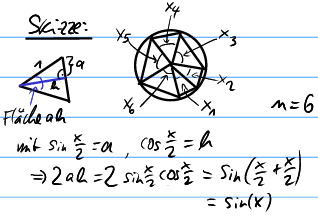
\includegraphics[width=5 cm,height=5cm]{bsp kap 9.10}
	\end{figure}\\
	\textbf{\underline{Lagrange-Ansatz:}} nur Stellen $x=(x_1,...,x_n)$ kommen für dieses Extremum in Frage, für die es einen Multiplikator $\lambda\in \mathbb{R}$ gibt mit $0=grad f(x)+\lambda grad f(x)=(\cos x_1,...,\cos x_n)+\lambda\cdot(1,...,1)$ was nur für $\cos x_1 =...=\cos x_n=0$ geht. Mit $0\leq x_j \leq \pi$ folgt $x_1=...=x_n,$ und aus der NB $g(x)=2\pi$ folgt $x_j=\frac{2\pi}{n}$ für $1\leq j\leq n$.\\
	Alsi ist der Flächeninhalt des einem Kreis einbeschrieben n-ecks genau für das regelmäßige n-Ecks maximal.\\
	\\
	\textbf{9.11. \underline{Motivation:}} $l,k\in \mathbb{N}, n=l+k, D\subset \mathbb{R}^n, f\in l^1(D,\mathbb{R}^k).$\\
	\begin{figure}[h]
		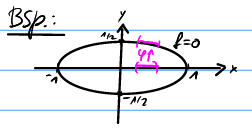
\includegraphics[width=5 cm,height=2.5cm]{bsp kap 9.11}
	\end{figure}\\
	Umkehrung? Ging für $\frac{\delta f}{\delta y}(a)\neq0$ bei $f:\mathbb{R}^1 x \mathbb{R}^1\rightarrow\mathbb{R}^1:$ dann findet sich eine Umgebung von a, in der f eine Umkehrfunktion besitzt.\\
	\\
	\textbf{9.12. \underline{Allgemeine Situation:}} Stelle $w=(a,b), (x,y)\in\mathbb{R}^l x \mathbb{R}^k=\mathbb{R}^{l+k}.$\\
	Dann: $f'(w)=(\frac{\delta f}{\delta y}(w), \frac{\delta f}{\delta y}(w))\in \mathbb{R}^{k x(l+k)} $\\
	\\
	\textbf{9.13\setulcolor{red}\ul{Satz über implizite Funktionen:}} $l,k \in \mathbb{R}^{j+k}, f\in l^1(D,\mathbb{R}^k)$\\
	\underline{Vor.:} $w\in D,F(w)=0, det(\frac{\delta f}{\delta y}(w))\neq 0 (w=(a,b)\in\mathbb{R}^lx\mathbb{R}^k).\\$
	\underline{Beh.:} $\exists U,V$ \setulcolor{green} \ul{$w\in U x V c \mathbb{R}^lx\mathbb{R}^k$} mit: \\
	\ul{$l:U\rightarrow V, x\rightarrow y \in V$ mit f(x,y)=0 ist eine Abbildung} und zwar 
	\ul{$l \in l^1 (U,\mathbb{R}^k)$.}\\
	Die Abbildung von l ist \ul{$l'(x)=*-(\frac{\delta f}{\delta y}\begin{pmatrix}x\\l(x)
		\end{pmatrix})^{-1}\frac{\delta f}{\delta x}\begin{pmatrix}
		x\\l(x)
	\end{pmatrix}$} $\in \mathbb{R}^{kxl}$.\\
	1.\underline{Bem.:} \ul{$f\in l^r$} $\xRightarrow{vollst. Ind}$ \ul{$l\in l^r$}.\\
	2.\underline{Bem.:} Bemerkenswert ist an diesem Satz, dass u.U. l nur schwierig berechnet werden kann, sehr wohl aber die Ableitung l'(x) nach der Formel (ohne die explizite Fkt. l ableiten zu müssen).\\
	\\
	\textbf{9.14.\underline{Bew.:}} $\bullet$ \underline{Falls} l existiert und diffbar, so gilt:\\
	\begin{equation}
		0=f(x,l(x))\Rightarrow (f(x,l(x)))'= 0\\
		\xRightarrow[]{K.R} \frac{\delta}{\delta x} f(x, l(x)) \cdot \frac{\delta x}{\delta x}+ \underbrace{\frac{\delta}{\delta y} f(x,l(x))}\cdot l'(x)=0\\
		\text{invbar, falls x nahe a, d.h. falls (x, l(x)) nahe (a,b)=w:}\\
		det\frac{\delta f}{\delta y}(w)\neq 0\Rightarrow det \frac{\delta f}{\delta y}(x,l(x))\neq 0\\
		\Rightarrow l'(x)=-(\frac{\delta f}{\delta y}(x, l(x))){-1} \frac{\delta f}{\delta x}(x, l(x))\Rightarrow l \in l^1.
	\end{equation} 
	$\bullet$\underline{Betr.}\begin{equation}
		F: D \rightarrow \mathbb{R}^lx\mathbb{R}^k, F\in l^1, (x,y)\rightarrowtail (x,f(x,y)).\\
		\text{Es gilt} F'(x,y)= \begin{pmatrix}
			I_l & 0\\
			\delta f & \delta f\\
			\delta x & \delta y
		\end{pmatrix} \in \mathbb{R}^{(l+k)x(l+k)}, det F' = det \frac{\delta f}{\delta y}\neq 0 \text{nahe w}.
	\end{equation}
	Der \setulcolor{blue}\ul{Satz über lokale Umkehrbarkeit 8.8} liefert nun:\\
	$\exists W,w \in W c  \mathbb{R}^lx\mathbb{R}^k:$\\
	\begin{align}
		\stackrel{\mathbb{R}^lx\mathbb{R}^k}{(x,y)}\rightarrowtail&\stackrel{\mathbb{R}^{l}x\mathbb{R}^k}{(x, f(x,y))}\rightarrowtail\stackrel{\mathbb{R}^lx\mathbb{R}^k}{(x,g(x,f(x,y)))}\\
		W\rightarrow& f(w)\xrightarrow{G=F^{-1}}W\xrightarrow{F}F(W)\\
		&(u,v)\rightarrowtail(u,\underbrace{g(u,v)}_{\in l^1})\rightarrowtail(u,\underbrace{f(u,g(u,v))}_{=v}),
	\end{align}\\
	d.h. \textcolor{blue}{(1)} g(x,f(x,y))=y\\
	\textcolor{blue}{(2)} f(x,g(x,y))=y.\\
	Wähle nun $U\subseteq \mathbb{R}^l$ mit $U x \{0\}\subseteq F(W)$, mit 0$\in\mathbb{R}^k.$\\
	(U existiert, da f(w)=0, also 0 als 2. Komponente in F(W) vorkommt.)\\
	Für $x \in U$ setze $l(x):= g(x,0).\\
	Denn: f(x,l(x))=f(x,g(x,0))=0.$\\
	Ferner: l ist eindeutig: $x\in U,f(x,y =0),$\\
	\textcolor{blue}{(1)}$\Rightarrow y = g(x,f(x,y))=g(x,0)=l(x).$\\
	\strut\hfill$\square$\\
	\textbf{9.15. \underline{Bsp.:}} Betr. $f(x,y)=x^2+y^2-1$. Für $y\textgreater0$ ist $y=\sqrt{1-x^2}$ die Fkt. y=l(x) "lokal", die durch f(x,y)=0 "implizit" gegeben ist.\\
	Laut Satz ist ihre Ableitung gleich $l'(x)=-\frac{2x}{2y}=-\frac{x}{\sqrt{1-x^2}}$ (wo $y\textgreater0$ ist),\\
	wir erhalten das Ergebnis direkt durch partielle Ableiten von f, ohne die explizite Funktion l(x) ableiten zu müssen. \textopencorner Was hier ginge.\textcorner\\
	\\
	\textbf{9.16. \underline{Bsp.:}} Ist die Glg. $x^y=y^x$ in der Nähe von a=(e,e) bzw. $\overline{a}=(2,4)$ nach einer der beiden Variablen auflösbar?\\
	Setze $f:\mathbb{R}^2_{\textgreater0}\rightarrow\mathbb{R}, f(x,y)=x^y-y^x,$ f ist für $x,y \textgreater0$ bel. oft diff'bar, $f(e,e)=f(2,4)=0.$ Die partiellen Ableitungen sind $D_1f(x,y)=yx^{y-1}-y^xln(y), D_2f(x,y)=x^yln(x)-xy^{x-1}.$\\
	$\bullet$ In (2,4) sind diese beiden partiellen Abl. $\neq 0$, also ist die Glg. dort lokal nach x oder y auflösbar (nur explizit nicht aber eben implizit!).\\
	Es gilt $l'(2,4)=-\frac{D_1f(2,4)}{2,4}=-\frac{2^5-2^5ln(2)}{2^4ln(s)-8}$ für die Ableitung der Auflösung nach y an der Stelle $\overline{a}=(2,4).$\\
	$\bullet$ In (e,e) gilt $f'(e,e)=grad f(e,e)=(0,0),$ der implizite Funktionensatz ist deswegen dort nicht anwendbar (und f dort nicht auflösbar nach x oder y).\\
	\\
	\textbf{9.17. \underline{Bem.:}} Gegeben sei die Situation wie in \blueul{9.3}, nähmlich:\\
	Sei $D\subset \mathbb{R}^n, 2 \leq l \leq n, (f_1,...,f_l)=f\in l^1(D,\mathbb{R}^l).$ Im gegebnsatz zu \blueul{9.4.} sei jetzt aber \\$rg\begin{pmatrix}
		D_1f_1&\cdots&D_nf_1\\
		\vdots&&\vdots\\
		D_1f_l&\cdots&D_nf_l
	\end{pmatrix}(a)$\greenul{=l}. Wegen \blueul{9.4} kann $f_{1rN}$ kein Extremum in $a\in N$ haben, analog auch nicht für $f_2,...,f_l$. Dann liegt eine besondere Situation vor, die in der mehrdimensionalen Analysis die folgende Beziehung hat.\\
	\\
	\textbf{9.18. \underline{Def.:}} $M\subseteq \mathbb{R}^n$ heißt \redul{(n-l)-dimensionale Untermannigfaltigkeit ("UMF")},\\
	(1) $M\cap U = U\cap f^{-1}(o)(=f^{-1}(o)), (2)rg Df(a)=l.$\\
	\\
	\textbf{9.19. \underline{Bem.:}} Jede \greenul{(n-l)-dim. UMF ist diffeomorph} zu $\underbrace{\{x\in \mathbb{R}^n;x_{n-l+1}=...=x_n=0\}}_{(n-l)-dimensionale Ebene im \mathbb{R}^n}$ der Dimension n-l\\	
\end{document}